\appendix
\renewcommand{\chaptername}{Phụ lục}
\chapter{Các tham số trong Diffusion}
 \label{appendix:Appendix1}

\section{Sự thay đổi của $\sqrt{\alpha}$ và $\sqrt{1 - \alpha}$}

\begin{figure}[H]
	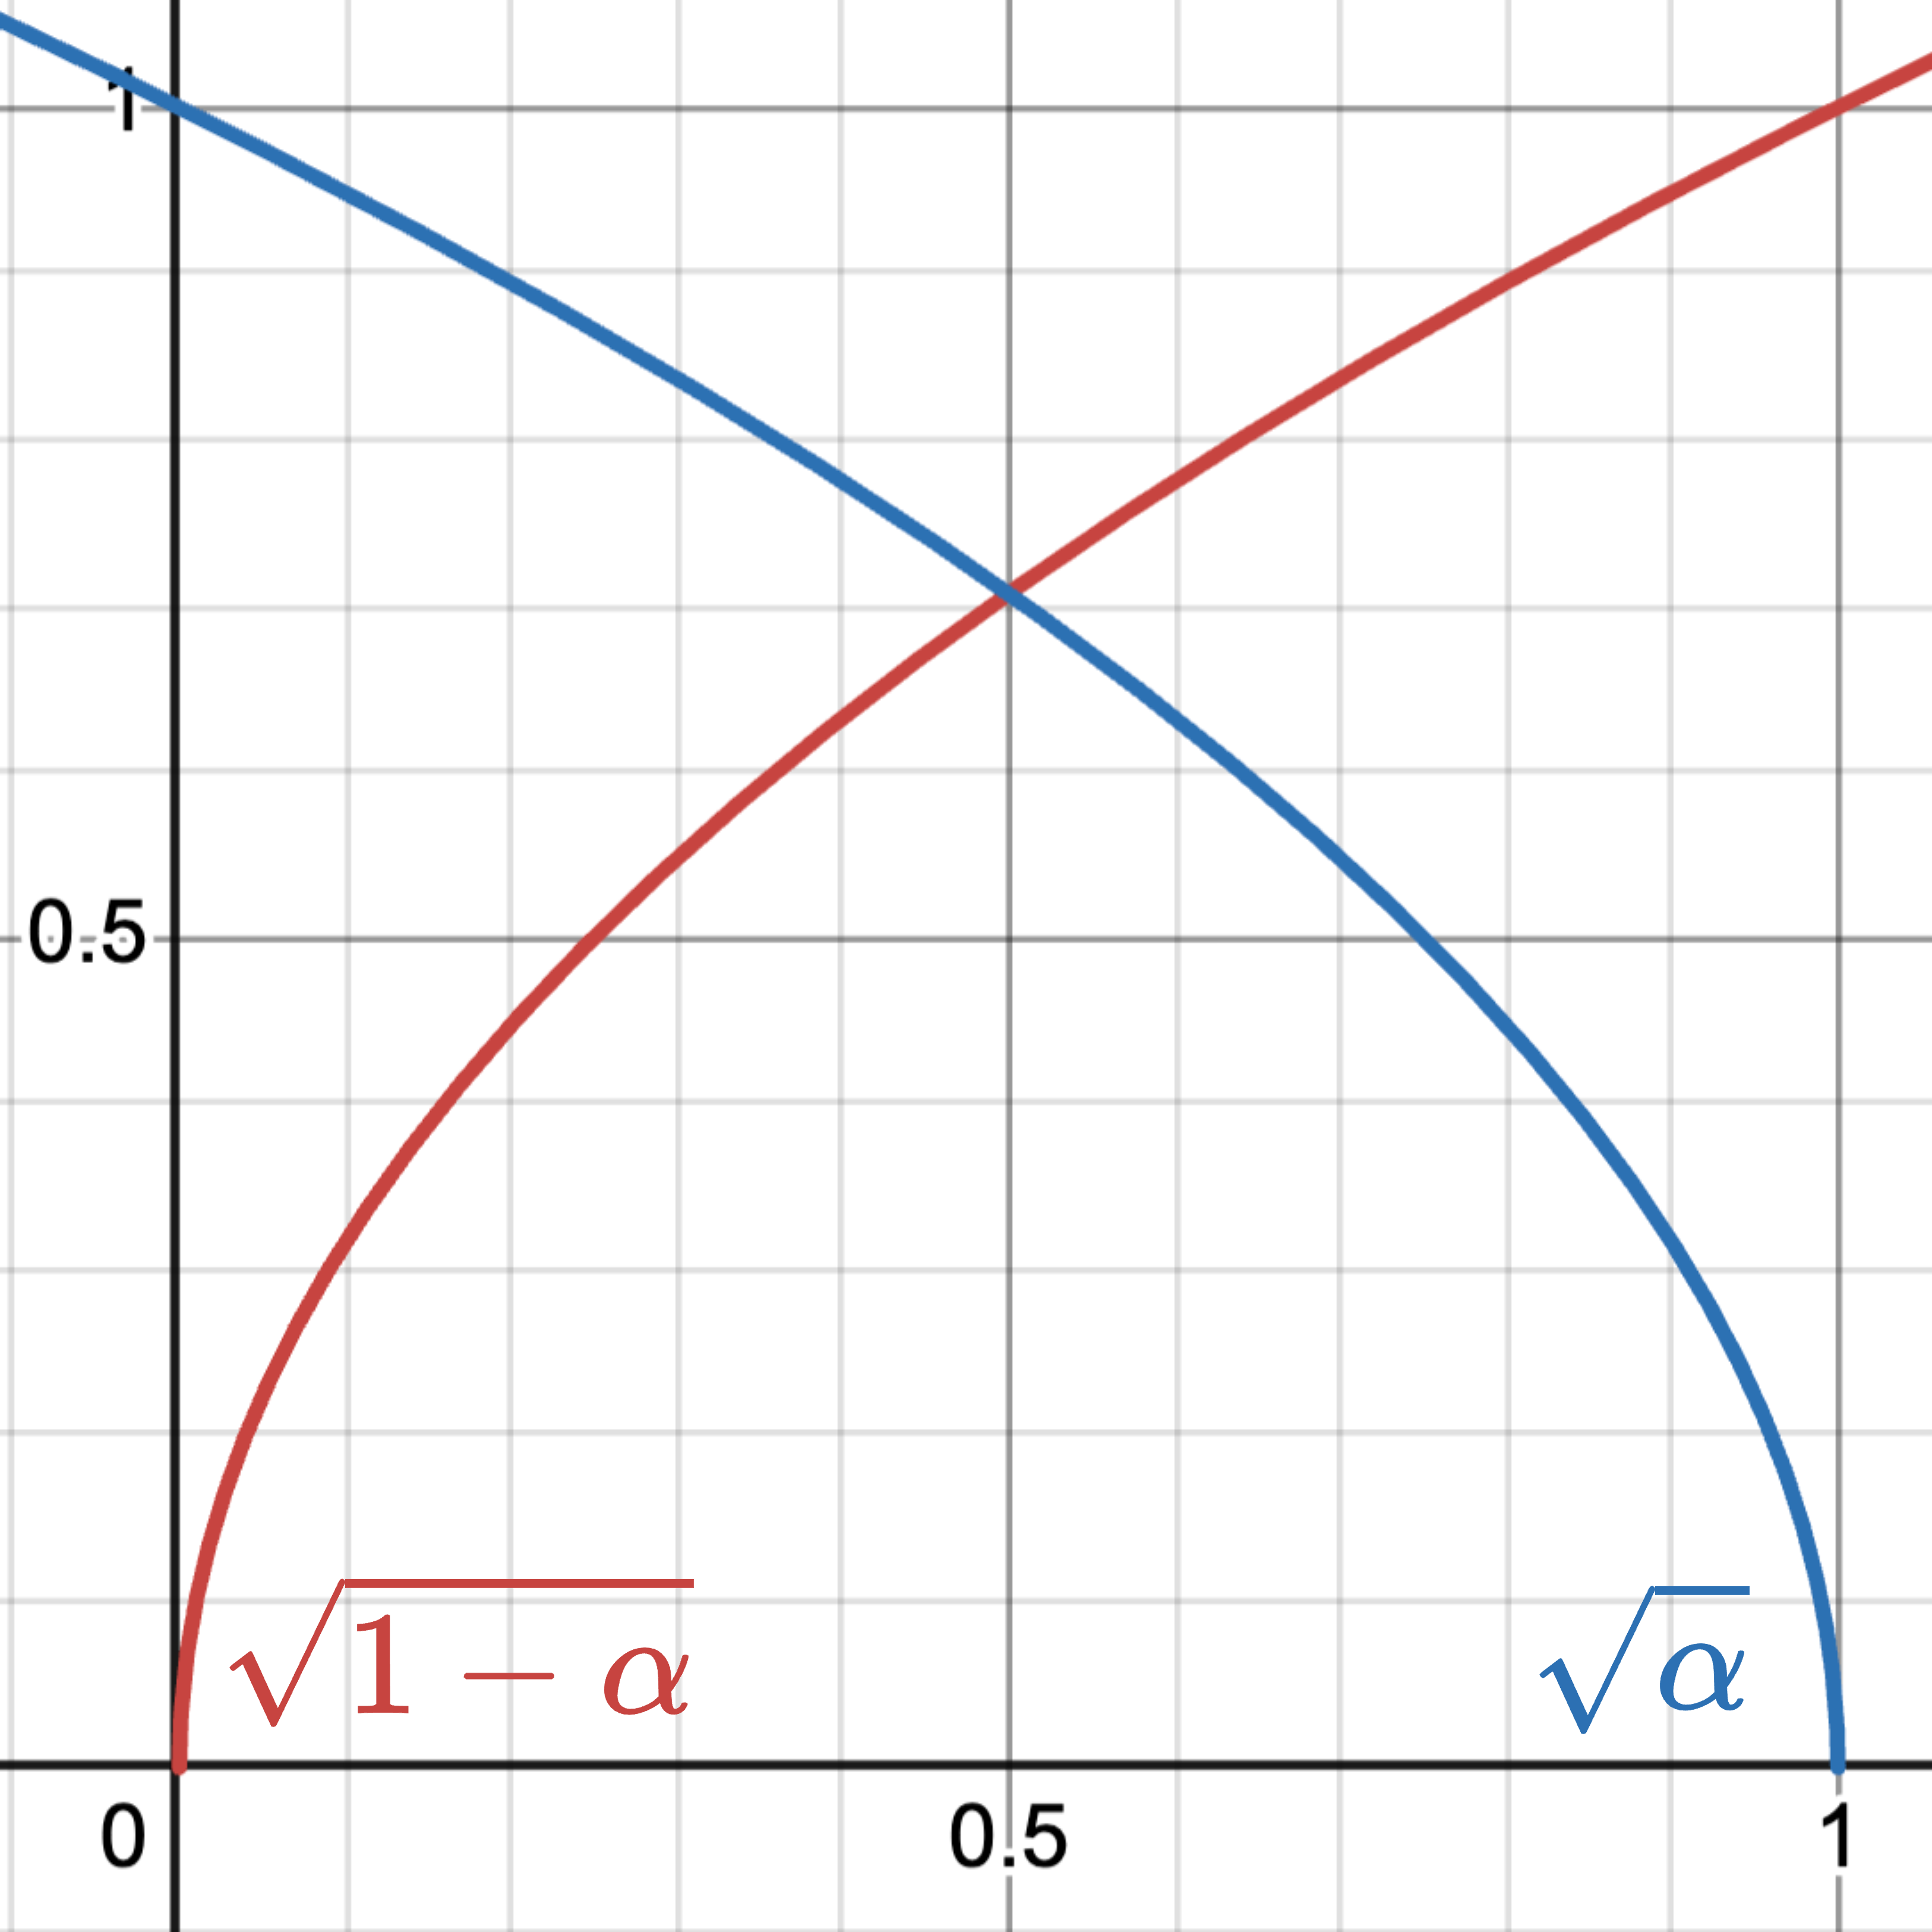
\includegraphics[width=0.5\linewidth]{SquareAlpha}
	\label{fig:wrapfig}
	\caption{Sự thay đổi của $\sqrt{\alpha}$ và $\sqrt{1 - \alpha}$}
\end{figure}

Trong quá trình diffusion, hệ thống muốn giảm dần sự hiện diện của $\bx$ và tăng dần sự hiện diện của nhiễu $\epsilon_t$. Với $\mathbf{x}_{t} = \sqrt{\alpha_t} \mathbf{x}_{t-1} + \sqrt{1 - \alpha_t} \epsilon_t$. Các hệ số $\sqrt{\alpha_t}$ và $\sqrt{1 - \alpha_t}$ giúp điều khiển quá trình này như sau:



\begin{itemize}
	\item $\sqrt{\alpha_t}$: Ban đầu giá trị lớn nhưng giảm dần để giảm sự ảnh hưởng vào kết quả tổng giữa nhiễu và $\bx_t$
	\item $\sqrt{1 - \alpha_t}$: Ban đầu giá trị nhỏ nhưng tăng dần theo từng bước. Với mục tiêu là đến cuối cùng thì sự ảnh hưởng của nhiễu càng lớn và trở thành nhiễu hoàn toàn.
\end{itemize}

Cả hai đại lượng này thay đổi theo thời gian trong quá trình diffusion, từ đó quyết định mức độ nhiễu được thêm vào từng bước $t$ và mức độ giữ lại trạng thái trước đó qua từng bước.


\section{Sự thay đổi của $\sqrt{\bar{\alpha}}$ và $\sqrt{1 - \bar{\alpha}}$}

$\bar{\alpha}_t = \prod_{i=1}^t \alpha_i$.  $\sqrt{1 - \bar{\alpha}_t} = \sqrt{1 - \prod_{i=1}^t \alpha_i}$. Cả $\sqrt{\bar{\alpha}}$ và $\sqrt{1 - \bar{\alpha}}$ đóng một vai trò quan trọng trong quá trình huấn luyện và sinh cử chỉ. Giúp kiểm soát mức độ nhiễu được thêm vào và cử chỉ, ta có thể thấy $\sqrt{\bar{\alpha}}$ giảm dần còn $\sqrt{1 - \bar{\alpha}}$ thì tăng dần..


\begin{figure}[H]
	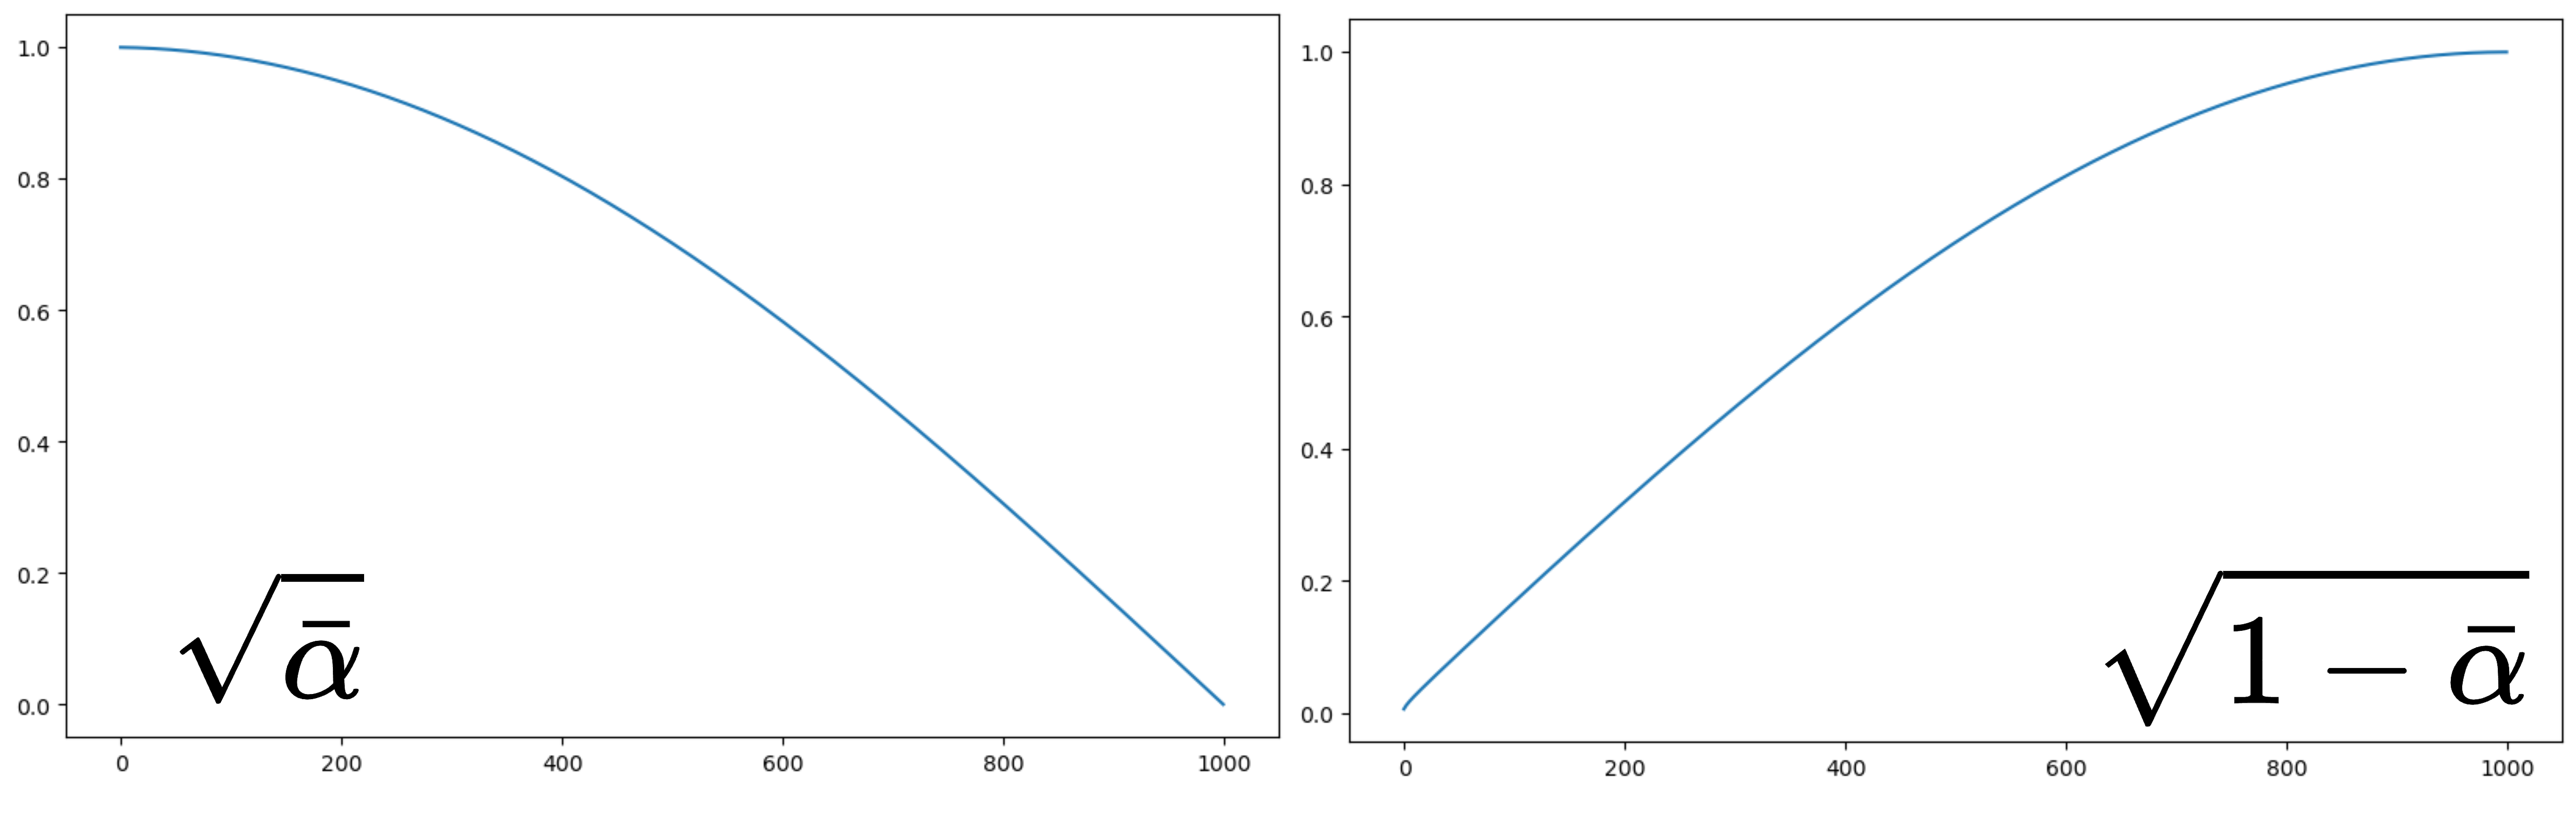
\includegraphics[width=\linewidth]{AlphaCumprod}
	\label{fig:AlphaCumprod}
	\caption{Quá trình thay đổi của $\sqrt{\bar{\alpha}}$ và $\sqrt{1 - \bar{\alpha}}$}
\end{figure}

%\section{So sánh $\epsilon$ objective và  $\bx_0$ }

\section{Sự thay đổi của $\sigma_t$}
 \label{appendix:Appendix1:NoiseScale}
\vspace{-10pt}
\begin{figure}[H]
	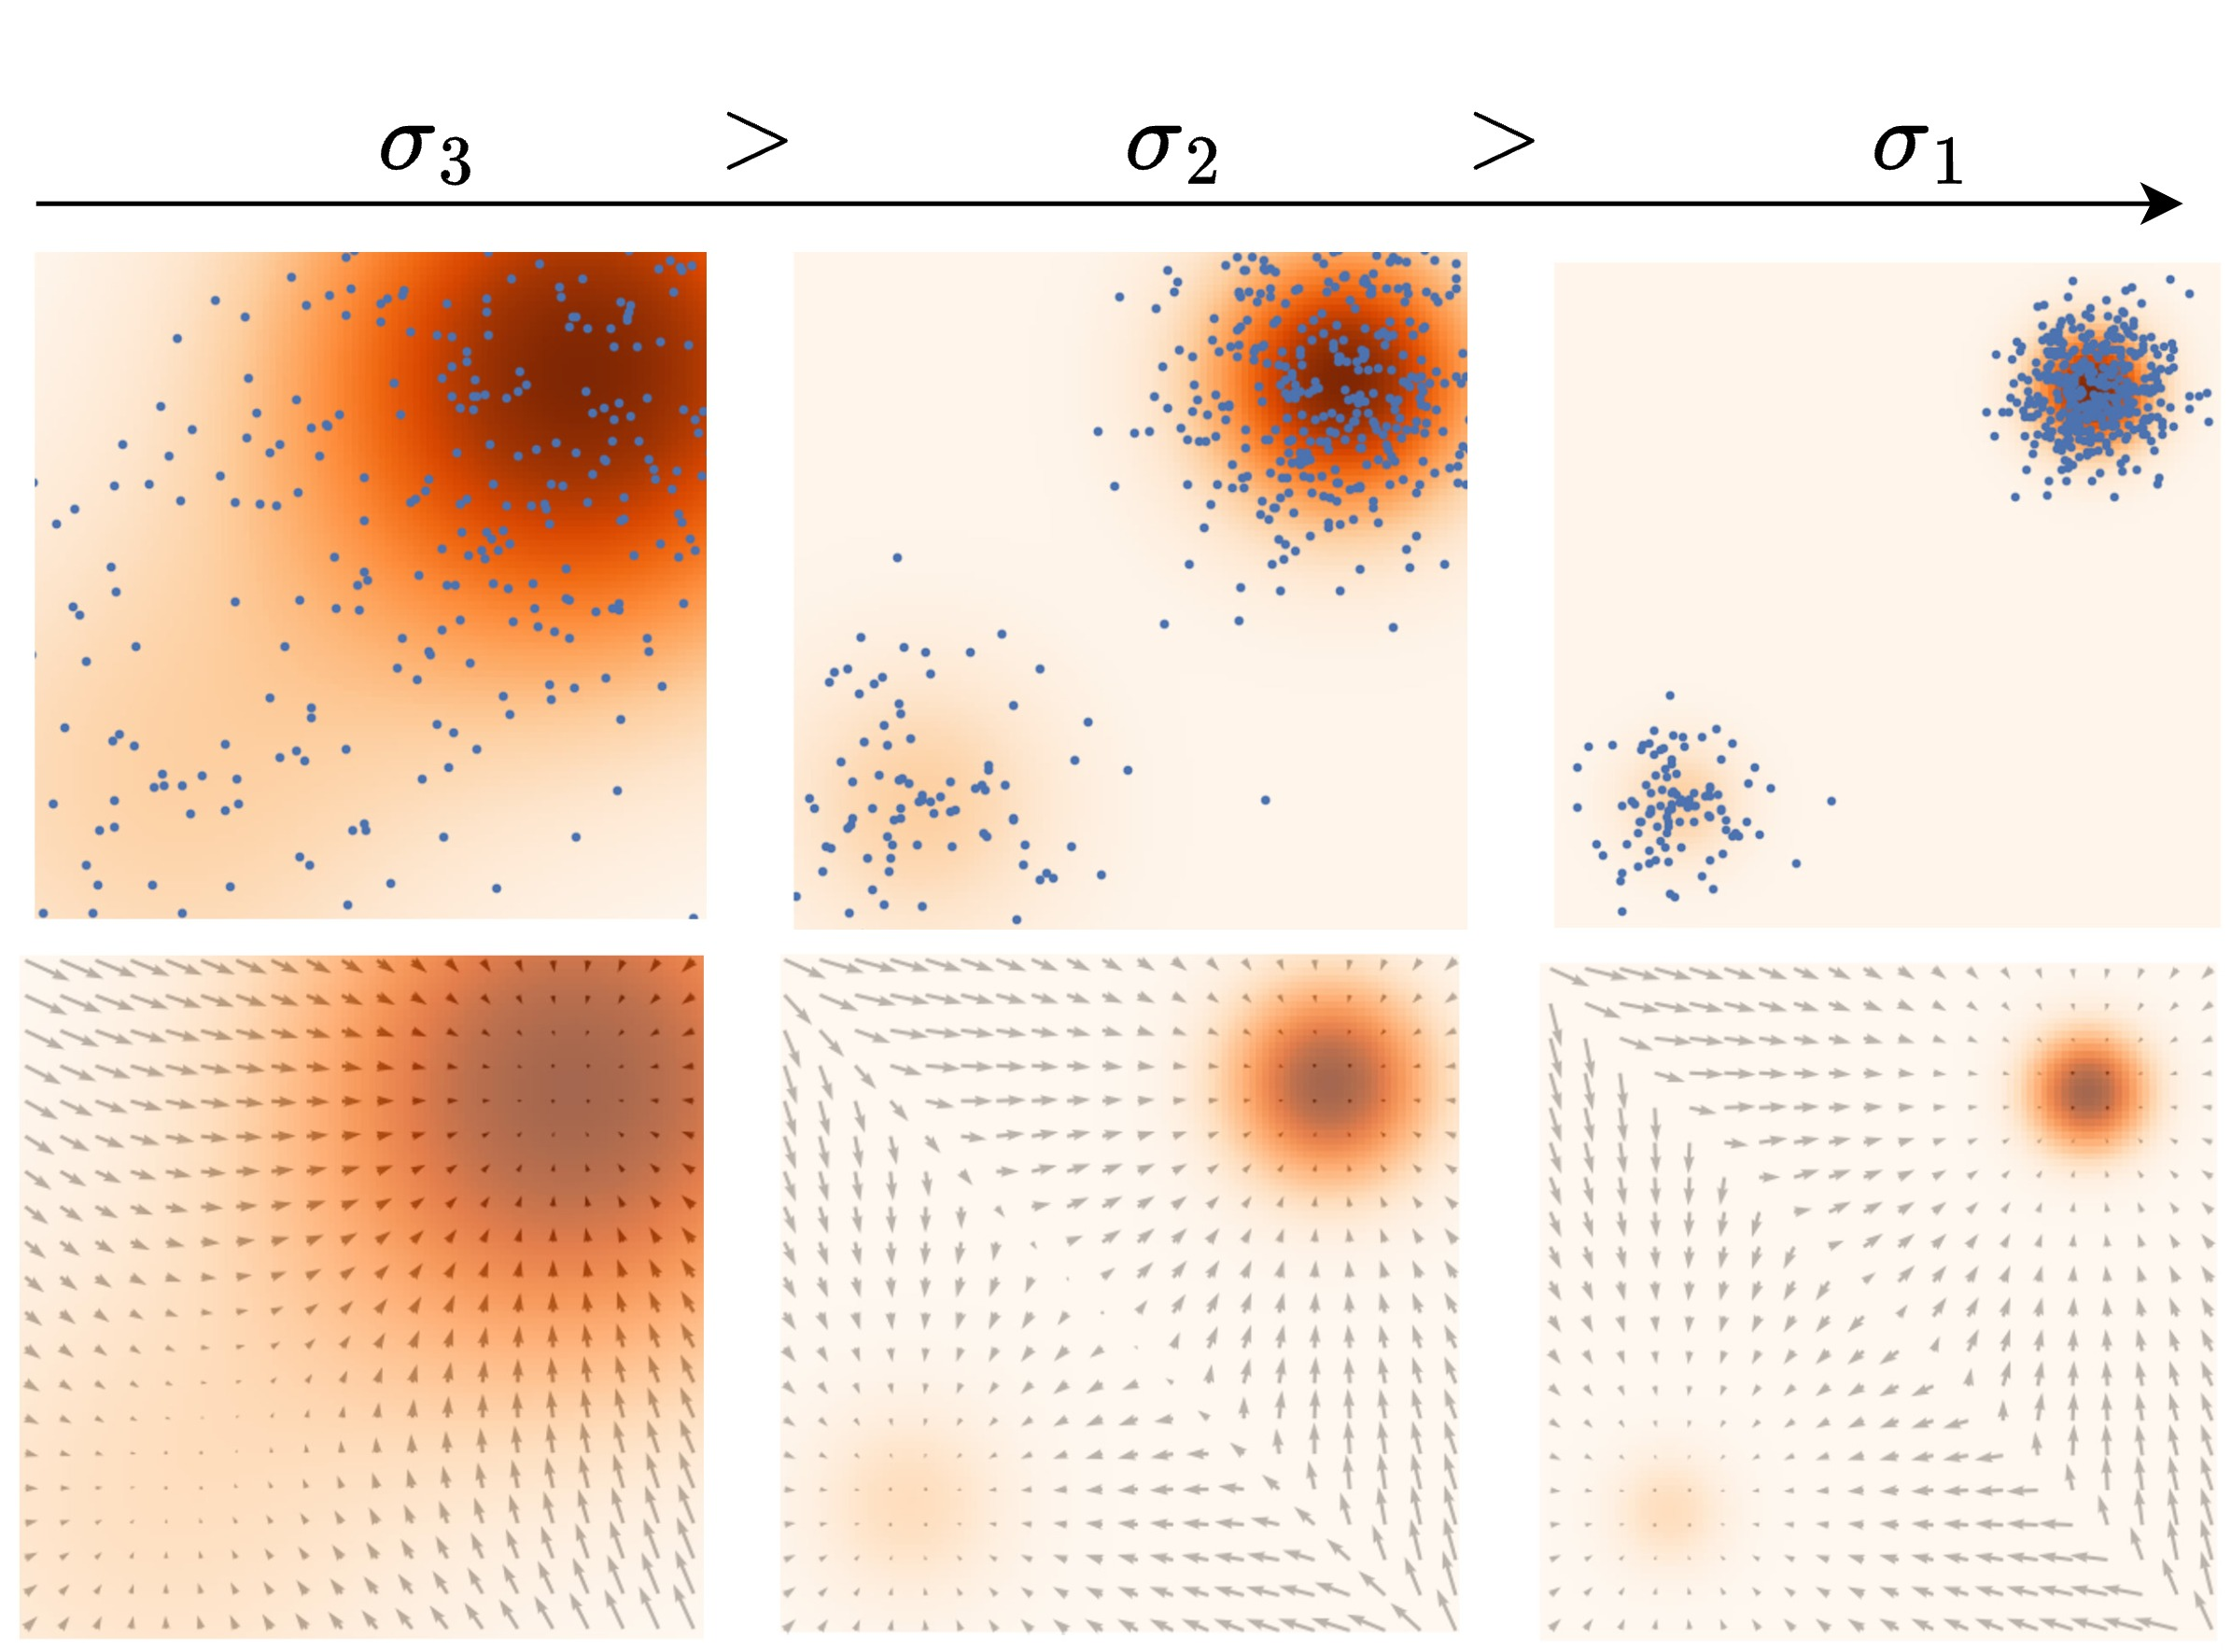
\includegraphics[width=\linewidth]{NoiseScale}
	\label{fig:NoiseScale}
	\caption{Sự thay đổi của hệ số $\sigma_t$ trong quá trình lấy mẫu }
\end{figure}
\vspace{-10pt}
Trong quá trình lấy mẫu, mục tiêu của việc giảm dần $\sigma_t$, mô hình có thể điều hướng về các vùng có mật độ dữ liệu cao ở từng bước $t$.

